% This is samplepaper.tex, a sample chapter demonstrating the
% LLNCS macro package for Springer Computer Science proceedings;
% Version 2.20 of 2017/10/04
%
\documentclass[runningheads]{llncs}
%
\usepackage{amssymb}
\usepackage{graphicx}
% Used for displaying a sample figure. If possible, figure files should
% be included in EPS format.
%
% If you use the hyperref package, please uncomment the following line
% to display URLs in blue roman font according to Springer's eBook style:
% \renewcommand\UrlFont{\color{blue}\rmfamily}

\begin{document}
%
\title{Sequence-Based Recommendation with Convolutional Bidirectional LSTM Network}
%
\titlerunning{CBLSTM for Sequence-Based Recommendation}
% If the paper title is too long for the running head, you can set
% an abbreviated paper title here
%
\author{Hailin Fu \and Jianguo Li\thanks{Corresponding
author.} \and Jiemin Chen \and Yong Tang \and Jia Zhu}
%
\authorrunning{H. Fu et al.}
% First names are abbreviated in the running head.
% If there are more than two authors, 'et al.' is used.
%
\institute{School of Computer Science, South China Normal University
\email{\{hailin,jianguo,,jzhu,XiaoDanyang,xqLin,ding\}@m.scnu.edu.cn}}
%
\maketitle              % typeset the header of the contribution
%
\begin{abstract}
With the rapid ongoing development of information technology, a variety of approaches can be applied in building recommendation systems, some of which have made impressive achievements in many different applications. To predict what a user will choose next given his consumed history is one of the crucial mission in recommendation. Most of traditional recommendation systems rely on much explicit feedback to produce output, but those methods often neglect the sequential relationship between datas. In this paper we propose an approach which is based on a bidirectional recurrent structure to capture the sequential feature of datas to promote the performance of next item recommendation. This is achieved by regarding this recommendation problem to a super multiply classification task. We collect consumed items of user in a sequence with time ascending order, and fit the model with last item as label, the rest items as features. Once trained well, the output layer will export the probabilities of items with given sequence. In the experiments, we compare our approach with several commonly used recommendation methods on a real-world dataset. Experimental results indicate that our sequence-based recommender can performance well for short-term interest prediction on a sparse, large, imbalanced dataset.

\keywords{Recommendation systems  \and bidirectional recurrent neural network \and deep learning.}
\end{abstract}
%
%
%
\section{Introduction}

There are two conditions for a successful application of personalized recommendation.
The first is the existence of information overload, if users can easily filter out their favorite ones from all the items, there is no need for personalied recommender. The second is that users do not have particularly clear demand for most of the time, because if the users have a clear need, they can directly through the search engine to find their interested items. 

With the rapid development of the Internet, in many kinds of fields, especially in shopping and entertainment, the number of products grow exponentially, which makes it difficult to retrieve and find the relevant thinks for users, therefore those users who have those needs are no doubt facing the problem of information overload. The prosperous researches of recommendation systems benefits a lot from the one million prize organized by Netflix\footnote{\url{www.netflix.com}}, a variety of impressive approaches for recommendation systems have been brought up after that competition. The main problems of recommendation systems faced with consist of two parts: ratings predicting and products recommendation. So to predict what a user will choose next is also a crucial task \cite{15}. In many websites and applications, such as online electronic business, news/videos website, music/radio station etc, them need a good service for users to recommend what they will like in future. We find that the sequence of datas implicits many interesting and relevant information, for example in a video website, user who watched "Winter is coming" (S01, E02 of Game of Thrones) will be more likely to watch "The Kingsroad" (S01, E02 of Game of Thrones). Even at the 2011 Recsys conference, Pandora\footnote{\url{www.pandora.com}}'s researchers gave a speech about music recommendation and said they find many users consumed music in sequences. However, to the best of our knowledge, few works use the sequential feature of datas to build recommender.

In the past few years, we have witnessed the tremendous prosperity of deep learning in Neural Language Processing, we noticed that recurrent neural network can capture the sequences of words in sentence. We also attempt  So in this paper we propose a novel recommendation model which uses bidirectional recurrent neural network to capture the sequences of user consumed datas. The main contributions of our work are as follows: 
 \begin{itemize}
\item This paper firstly introduce Convolutional bidirectional Long Short-Term Memory(CbLSTM) network to the domain of Recommendation System. 
\item We propose a novel Sequence-based recommendation framework with deep neural network, which can capture the sequential features of datas, as well scales linearly with the number of objectives (both of users and items).
 \end{itemize}

The reset of the paper is organized as follows. Related work is discussed briefly in Section 2. In Section 3, we introduce the overall recommendation framework in detail. Section 4 introduces the experiments, we compare our proposed method with the traditional recommendation methods on the same real-world dataset. Finally we conclude this paper in Section 5, and point out some future work.

\section{Related Work}
\subsection{Traditional methods in recommendation}

There are three main classes of traditional recommendation system. Those are collaborative filtering systems, content-based filtering systems and hybrid recommendation systems \cite{12}. Collaborative filtering \cite{1,2,3,4} systems generate recommendations based on crowd-sourced input. They recommend for user according to find similar user group, analysis those similar users’ rating for certain item, to generate preference prediction for this user in special products. Collaborative filtering algorithm can be generally classified into Memory-based \cite{1,2} collaborative filtering and Model-based \cite{3,4,5}collaborative filtering. Memory-based collaborative filtering include User-based collaborative filtering \cite{1} which evaluate the similarity between users by different users’ ratings on the item, making recommendations based on the similarity between users and Item-based collaborative filtering \cite{2} which evaluate the similarity between items by the user’s rating on different items, making recommendations based on the similarity between items. Model-based CF algorithm mainly uses the rating information to train corresponding model, and use this model to predict unknown data. These mainly include Bayesian networks \cite{3}, clustering models \cite{4}, Probabilistic Matrix Factorization \cite{5}. Content-based systems \cite{6} generate recommendations for users based on a description of the item and a profile of the user’s preference. Hybrid recommendation systems \cite{7} combine both collaborative and content-based approaches, they help improve recommendations that are derived from sparse datasets.

\subsection{Deep learning in recommendation}
Deep learning is able to efficiently capture unstructured data, such as auditory and visual information, and extract more complex abstractions into higher level data representation \cite{20}. Dieleman et al. \cite{8} proposed a content-based recommender system which used CNN to extract audio signal for Spotify Music. Shumpei et al. \cite{9} presented a RNN based news recommender system for Yahoo News. Covington et al. \cite{10} use historical query, demographic and other contextual information as features, presented a deep neural network based recommendation algorithm for video recommendation on YouTube. Hidasi, Balázs, et al. \cite{11} presented a Session-based recommendations with RNN. Wan, Shengxian, et al. \cite{15} also proposed using RNN to build a next basket recommendation.

\section{Proposed Approach}

In the area of Natural Language Processing, many researches have shown that a remarkable highlight for Text Classification can be achieved by learning sequences of words \cite{21}. Our work inspired by previous study of Siwei Lai et al. \cite{13}, where a neural network is proposed to capture the semantics of the text. We took a similar approach by considering each item as a word, the catalog of items as the full vocabulary, and a sequence of the historical consumed items of one user as a sample document. Our model consists of four layers: embedding, recurrent structure, pooling layer and output layers. We use this model to capture the sequence feature of the user's consumed datas. Figure 1 shows the structure of our sequence-based recommender.
\begin{figure}[htbp]
\centerline
{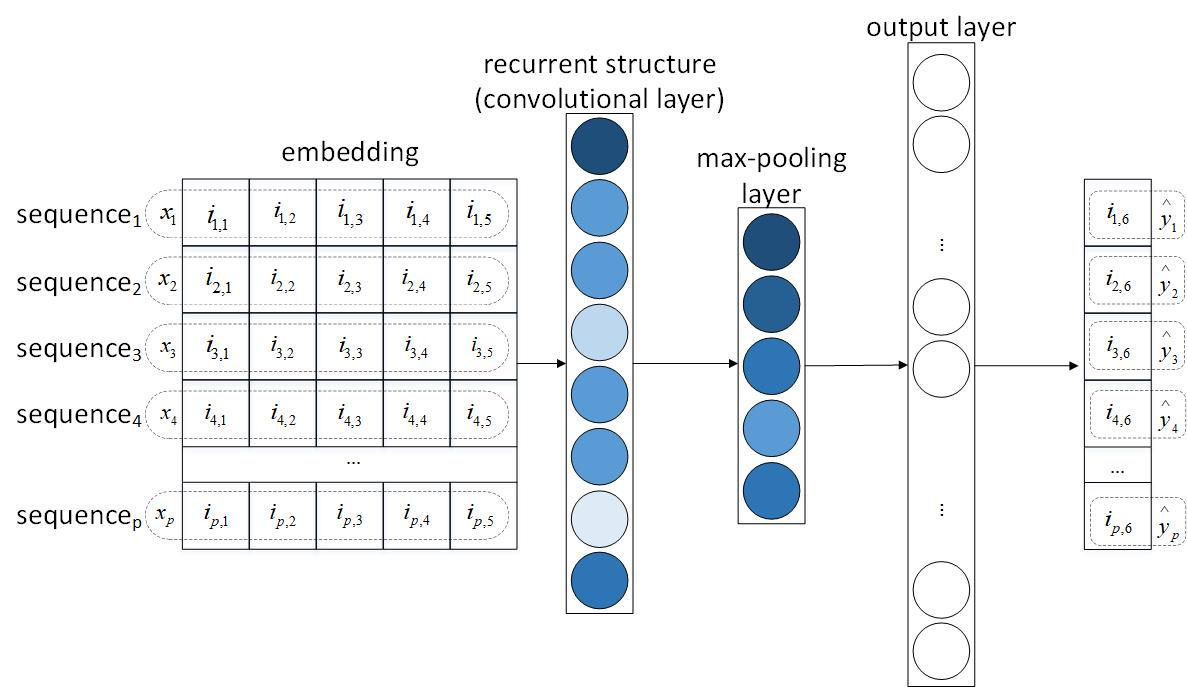
\includegraphics[height=6.2cm,width=\linewidth]{structer.jpg}}
\caption{Framework of sequence-based recommendation }
% \label{fig}
\end{figure}
\subsection{Notations }\label{AA}
Let us assume that $\mathbb{U}= \left \{ u_{1},u_{2},...,u_{N} \right \}\label{eq}$ be the user set and $\mathbb{I}= \left \{ i_{1},i_{2},...,i_{M} \right \}$ be the item set. For each user $u$, there is a observed consumed items sequence $S_{u}=\left \{ I_{u}^{1},I_{u}^{2},...,I_{u}^{t-1},I_{u}^{t} \right \}$ in ascending order of time, where $I_{u}^{t}$ is the item consumed by user $u$ at time $t$. The sequential prediction problem is to predict $I_{u}^{t+1}$ for each user $u$, using given $S_{u}$ at time $t+1$.

The input of the network is a sequence $S_{u}=\left \{ I_{u}^{1},I_{u}^{2},...,I_{u}^{t-1},I_{u}^{t} \right \}$, which contain consumed items of each user. We consider any item can appear only once in the history of any user. Therefore model could recommend items that the user had not yet selected. The output of the network is a softmax layer with a neuron for each item in the catalog. We use $p(k|S,\theta )$ to represent the probability that user $u$ who had a historical consumed items sequence $S$ would select item $k$ at next time, where $\theta$ is the parameter in the network.

\subsection{Embedding layer}
 We use the latest sequences of user consumed items as the features, and the last item as the label, to built a super multiply classification supervised learning model. So in the period of the feature engineering, we need to convert the features into vectors and map them with labels. One-hot vector representation is the most common method to discrete every item. However, One-hot encoded vectors are high-dimensional and sparse. If we use One-hot encoding to deal with 1000 items, each item will be represented by a vector containing 1000 integers, 999 of which are zeros. In a big dataset this approach is unacceptable considering computational efficiency. Word Embedding shines in the field of Natural Language Processing , instead of ending up with huge One-hot encoded vectors we also can use an embedding matrix to keep the size of each vector much smaller:
 \begin{equation}
e(I_{i})=EI_{i}
\end{equation}
where $E\in \mathbb{R}^{|e|\times |M|}$, $|e|$ is the size of the embedding layer, $|M|$ is the number of items in the database. So $e(I_{i})$ is the embedding of consumed item $I_{i}$, which is a dense vector with $|e|$ real value elements.

\subsection{User Short-term Interest Learning}
We combine a user consumed item $I_{u}^{t}$ and other items previous and subsequent $I_{u}^{t}$ to present the current interest of user $u$ at time $t$. The behavior sequences help us to indicate a more precise short-term interest of user. In this recommender, we use a recurrent structure, which is a bidirectional recurrent neural network, to capture the short-term interest of the user.

We define $h_{b}(I_{i})$ as the user's interest before consuming a item $I_{i}$ and $h_{a}(I_{i})$ as the user's interest after consuming a item $I_{i}$. Both $h_{b}(I_{i})$ and $h_{a}(I_{i})$ are dense vectors with $|h|$ real value elements. The interest $h_{b}(I_{i})$ before item $I_{i}$ is calculated using Equation (1). $W^{(b)}$ is a matrix that transform the hidden layer (interest) into the next hidden layer. $W^{(cb)}$ is a matrix that is used to combine the interest of the current item with the next item's previous interest. $\sigma $ is a non-linear activation function. The interest $h_{a}(I_{i})$ after consuming item $I_{i}$ is calculated in a similar equation. Any user's initial interest uses the same shared parameters $h_{b}(I_{1})$. The subsequent interest of the last item in a user's history share the parameters $h_{a}(I_{n})$.
\begin{equation}
h_{b}(I_{i})=\sigma (W^{(b)}h_{b}(I_{i-1})+W^{(cb)}e(I_{i-1}))
\end{equation}
\begin{equation}
h_{a}(I_{i})=\sigma (W^{(a)}h_{a}(I_{i+1})+W^{(ca)}e(I_{i+1}))
\end{equation}
where the initial interest $h_{b}(I_{1}),h_{a}(I_{n})\in \mathbb{R}^{|h|}$, $W^{(b)},W^{(a)}\in \mathbb{R}^{|h|\times |h|}$, $W^{(cb)},W^{(ca)}\in \mathbb{R}^{|e|\times |h|}$.

As shown in Equation (2) and (3), the interest vector captures the interest in user's previous and subsequent behavior. We define the temporary status of interest when user taking a behavior $I_{i}$ as the Equation (4) shown. This manner concatenate the previous temporary status of interest $h_{b}(I_{i})$ before user consuming item $I_{i}$, the embedding of behavior $I_{i}$ consumed item $e(I_{i})$, and the subsequent temporary status of interest $h_{a}(I_{i})$ after user consuming item $I_{i}$
\begin{equation}
x_{i}=[h_{b}(I_{i});e(I_{i});h_{a}(I_{i})]
\end{equation}
So using the consumed behavior sequences $\left \{ i_{1},i_{2},...,i_{n-1},i_{n} \right \}$, if our model learned the temporary interest status $x_{n-1}$, users who consumed item $i_{n-1}$ would have bigger probability to get a recommended item $i_{n}$. The recurrent structure can obtain all $h_{b}$ in a forward scan of the consumed items sequences and $h_{a}$ in a backward scan of the consumed items sequences. After we obtain the representation $x_{i}$ of the temporary status of interest when user taking a item $I_{i}$, we apply a linear translation together with the $tanh$ activation function to $x_{i}$ and send the result to the next layer.
\begin{equation}
y_{i}^{(2)}=tanh(W^{(2)}x_{i}+b^{(2)})
\end{equation}
where $W^{(2)}\in \mathbb{R}^{H\times (|e|+2|h|)}$, $b^{(2)}\in \mathbb{R}^{H}$ are parameters to be learned, $H$ is the recurrent layer size, $y_{i}^{(2)}$ is a latent interest vector, in which each interest factor will be analyzed to determine the most useful factor for representing the users consumed items sequences.

\subsection{Popularity Trend Learning}
When all of the sequences of user's consumed items are calculated, we apply a max-pooling layer.
\begin{equation}
y^{(3)}=\max_{i=1}^{n}y_{i}^{(2)}
\end{equation}
Max pooling is done by applying a max filter to non-overlapping subregions of the upper representation. With the pooling layer, the number of parameters or weights within the model reduced rapidly, which could reduce the spatial dimension of the upper input volume drastically and lessen the computation cost. We could capture the attribute throughout the entire sequence and find the most popular sequences combination in the whole users' history using the max-pooling layer. The last part of our model is an output layer as following:

\begin{equation}
y^{(4)}=W^{(4)}y^{(3)}+b^{(4)}
\end{equation}
where $W^{(4)}\in \mathbb{R}^{O\times H}$, $b^{(4)}\in \mathbb{R}^{O}$ are parameters to be learned, $O$ is the convolutional layer size.

Finally, a softmax activation function is applied to $y^{(4)}$, which can convert the output values to the probabilities of next items. 

\begin{equation}
p_{i}= \frac{e^{y_{i}^{(4)}}}{\sum_{k=1}^{n}e^{y_{k}^{(4)}}}
\end{equation}

\begin{figure}[htbp]
\centerline{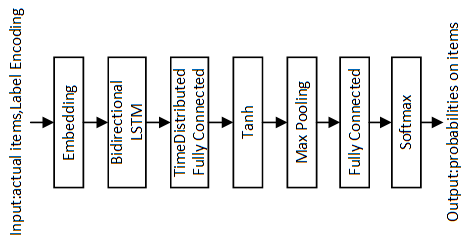
\includegraphics[width=8.5cm,height=3.5cm]{model.png}}
\caption{Illustration of model structure.}
\label{fig}
\end{figure}
\subsection{Training}

We define all of the parameters to be trained as $\theta $.
\begin{equation}
\theta=  \left \{ E,b^{(2)},b^{(4)},h_{b}(B_{1}),h_{a}(B_{n}),W^{(2)}, W^{(4)},\right.\\
\left.W^{(b)},W^{(a)},W^{(b)},W^{(cb)},W^{(ca)} \right \} \\
\end{equation}
The training target of the network is to minimize the categorical cross entropy loss:
\begin{equation}
\mathcal{L}(y,S,\theta )=-\sum_{u\in \mathbb{U}}y_{u}\log p(y|S_{u},\theta)+(1-y_{u})\log (1-p(y|S_{u},\theta ))
\end{equation}
\subsection{Time Complexity Analysis}

In that sequence-based recommendation model, the calculation process mainly includes following steps: Embedding, Recurrent structure, Max-pooling and output.

Firstly, our embedding layer creates an embedding matrix, the shape of embedding matrix is only related to the number of items and length of latent factor $|e|$. So the time complexity in the first step is $O(n)$. Secondly, the embedding matrix will be transported to a Recurrent Neural Network structure, We use a bi-directional Long Short-Term Memory (LSTM) structure in this layer, LSTM is a variant of Recurrent Neural Network \cite{22}. For every sequence, the bi-directional LSTM structure will apply a forward and a backward scan, and based on the citation [14], the time complexity of the bi-directional LSTM we can know is $O(n)$. Thirdly, the output of the bi-directional LSTM will be transported to the pooling layer, the time complexity of the pooling layer is also $O(n)$. The overall model is a cascade of those layers, therefore, our sequence-based recommendation model appears a time complexity of $O(n)$, which is linearly correlated with the number of sequences. The overall time complexity of the model is acceptable, so that big datas can be effectively processed.


\section{Experiments}


\subsection{Dataset}

In order to verify our approach is feasible, we perform experiments on a real-world dataset: LiveStreaming dataset, which collected users' transaction datas from a live streaming website in China. Each line in LiveStreaming records a sequence of browsed items of a user in ascending order of time.  The initial collected LiveStreaming dataset cotains 1806204 lines, which means that contacts 1806204 unique users. The length of each line ranges from 1 to 1060. Total 541772 different items contained in that dataset. We remove those users which are annotated by less than 15 items then randomly select 10 thousands users as the experimental part denoted as LiveStreaming-10M. Finally, 10000 users and 12292 items contains in LiveStreaming-10M. We split 80\% of this part into training set, and keep the remaining 20\% as the validation set. 

\subsection{Evaluation and Metrics}

As a recommendation model, we will recommend top N item(s) for each user, denoted as $\hat{I}_{u}^{t+1}$. We adopt $Precision@N$, $Recall@N$ scores to evaluate our model and baseline models. We can define the measures as follows Eqs. 11, 12:

\begin{equation}
Precision@N=\frac{\sum_{u}|\hat{I}_{u}^{t+1}\cap I_{u}^{t+1} |}{\left | \mathbb{U} \right |*N}
\end{equation}

\begin{equation}
Recall@N=\frac{\sum_{u}|\hat{I}_{u}^{t+1}\cap I_{u}^{t+1} }{\left |\sum_{u}|I_{u}^{t+1}| \right |}
\end{equation}
In order to get a harmonic average of the precise and recall, the $F1@N$ score was measured here, where a higher F1 score reaches, a more effective result gets, which is shown as Eqs. 13:

\begin{equation}
F1@N=\frac{2\times Precision@N\times Recall@N}{Precision@N+Recall@N}
\end{equation}
\subsection{Training}

We conduct the experiments on a personal computer, the runtime environment of our experiments is: 2.80GHz Inter Core i7 CPU, NVIDIA GeForce GTX 1050 GPU, 8G memory, 256G storage and Windows 10 operating system.

Our model is implemented on Keras, an open-source deep learning framework, using TensorFlow-gpu backend, so we can train our model with GPU acceleration. We use stochastic gradient descent (SGD) \cite{22} with an initial learning rate $\alpha$ as 0.01 to optimize neural network parameters, at each iteration with a given example, SGD finds the direction where the objective function can be slashed quickest, fewer state-of-the-art neural networks using the vanilla version. A set of technics have been developed to speed up training, \textbf{momentum update} \cite{22} is a commonly used acceleration approach in gradient descent method, here we use momentum $\beta $ as 0.9. The stochastic gradient descent with momentum updates are computed in the following way:

\begin{equation}
x_{t+1} = x_{t} + \beta \ast v -\alpha \ast dx
\end{equation}
Where $v$ is the vector of parameters, $dx$ is the gradient of the object function. With Momentum update, the parameter vector will build up velocity in any direction that has consistent gradient.

When training deep networks, it is usually helpful to anneal the learning rate over time. A high learning rate helps decay the loss faster, but it may be unable to roll down into the deepest smoothly. We also use a \textbf{decay} \cite{22} of $1\times 10^{-4}$ for decreasing learning rate after each iteration. The learning rate $\alpha$ updates are computed in the following way:
\begin{equation}
\alpha = \alpha * \frac{1}{1 + decay * iterations}
\end{equation}

Another training tip we use to save training time and avoid overfitting is \textbf{EarlyStopping} \cite{22}, the mechanism behind EarlyStopping is we set a monitor on the loss of validation set, if the loss of validation set doesn't get reduced within three iterations, which indicates networks have been trained over.

The other hyper-parameters like hidden layer size and embedding layer size we use those most common values firstly,
in order to get best performance on that dataset, we tune hyper-parameters by fixed others and adjusting only one in every training. After several cumbersome tuning, we get the following other hyper-parameters: embedding layer size $|e|$ = 100, recurrent layer size $H$ = 200, convolutional layer size $O$ = 100, batch size as 32 and initial number of epochs as 100.
\begin{figure}[htbp]
\centerline
{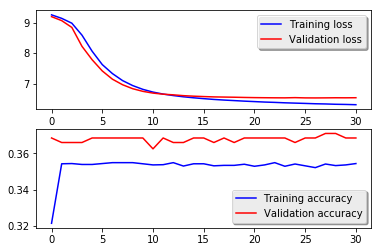
\includegraphics[height=6.2cm]{10thousand@6.png}}
\caption{CbLSTM training on 80\% LiveStreaming-10M with Time Windows as 5, and recommends items with the top 20 probability values}
\label{fig}
\end{figure}

We also explore how many datas the CbLSTM model needs for every user to learn the global sequences tendency and make a good recommendation, so we design a experiment using LiveStreaming-10M with different Time Windows ranges from 1 to 10. When Time Windows equals to 2, means we only use the last item in sequence as label, the latest one item as feature to fit our model. 
\begin{figure}[!htb]
   \begin{minipage}{0.48\textwidth}
     \centering
     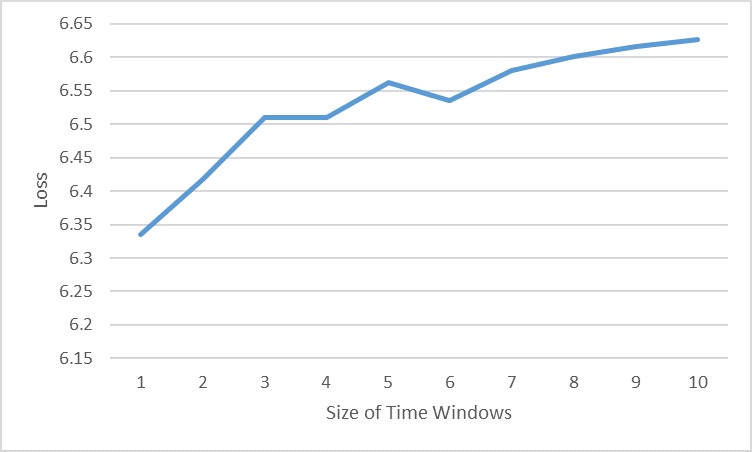
\includegraphics[width=\linewidth]{Loss_timewindows.png}
     % \caption{Interpolation for Data 1}
     % \label{Fig:Data1}
   \end{minipage}\hfill
   \begin {minipage}{0.48\textwidth}
     \centering
     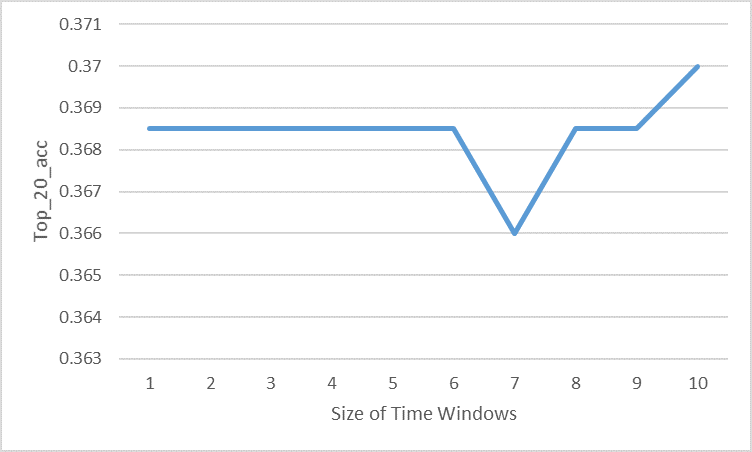
\includegraphics[width=\linewidth]{Top_20_acc_timewindows.png}
     % \caption{Interpolation for Data 2}
     % \label{Fig:Data2}
   \end{minipage}
   \caption{The training results of CbLSTM model on 80\% LiveStreaming-10M with different Time Windows}
   % \label{fig:coffee}
\end{figure}


\subsection{Compared Algorithms}
In this paper, We compare our model with several existing baselines, and the state-of-the-art approaches in the area of recommendation system:

 \begin{itemize}
\item \textbf{POP}: Popularity predictor that always recommends the most popular items of the training set, it feedbacks the global popularity. Despite its simplicity it is often a strong baseline in certain domains.
% \item \textbf{T-POP}: This baseline recommends the most popular items at the current moment.
\item \textbf{IBCF}: Collaborative Filtering is one of the most classical method of recommendation, which includes Item-based Collaborative Filtering (IBCF) \cite{2}and User-based Collaborative Filtering (UBCF \cite{1}, both yet still strong baselines for top-N recommendation. User-based collaborative filtering which evaluate the similarity between users by different users’ ratings on the item, recommending those items for user consumed by his similar users but not yet consumed by him. However, not every dataset for recommendation contains users' ratings information, in this task, we set the rating 1 if user consumed the corresponding item, or 0 if not. Similarity between $u_{i}$ and $u_{j}$ was measured using cosine angle:
\begin{equation}
sim(u_{i},u_{j})=\cos (\vec{u_{i}},\vec{u_{j}})=\frac{\vec{u_{i}}\cdot \vec{u_{j}}}{\left \| \vec{u_{i}} \right \|_{2}\ast \left \| \vec{u_{j}} \right \|_{2}}
\end{equation}

\item \textbf{UBCF}: User-based Collaborative Filtering which evaluate the similarity between items by different users’ ratings on the item, recommending items similar to those items consumed already for user. In UBCF, we also use cosine angle to measure similarity between items.
% \item \textbf{PMF}: 
% \item \textbf{Apriori}:
\end{itemize}

\begin{table}[htbp]
\begin{center}
\begin{tabular}{|c|c|c|c|c|}
\hline

\textbf{Metrics} & \textbf{POP}& \textbf{UBCF}& \textbf{IBCF}& \textbf{CbLSTM} \\
\hline
Precision@1& 0.0056& 0.0108 & 0.0112 & 0.1135 \\
\hline
Recall@1& 0.0056& 0.0108 & 0.0112 & 0.1135\\
\hline
F1@1& 0.0056& 0.0108 & 0.0112 & 0.1135\\
\hline
Precision@5& 0.00018& 0.0476 & 0.00626 & 0.0463\\
\hline
Recall@5& 0.0009& 0.0476 & 0.0313 & 0.2315\\
\hline
F1@5& 0.0003& 0.0476 & 0.010433333 & 0.07716666666666668\\
\hline
Precision@20& 0.00015& 0.1154 & 0.004705 & 0.018425\\
\hline
Recall@20& 0.003& 0.1154 & 0.0941 & 0.3685\\
\hline
F1@20& 0.000285714& 0.1154 & 0.008961905 & 0.035095238095238096\\
\hline
\end{tabular}
\label{tab1}
\end{center}
\caption{When the length of recommendation list is 1,5,20 respectively, we compare different approaches using LiveStreaming-10M dataset with Time Windows as 5}
\end{table}

Our experiments firstly compare CbLSTM model with itself in different length of sequence. From the Fig.4 we can conclude that our sequence-based recommendation with CbLSTM also can make recommendations for someone even though with a little information about him. Our approach provides a way to solve the famous cold start problem for recommendation system. Furthermore, from the results (Tab. 1), we can see that the performances of our approach are consistently better than other traditional recommendation baselines on this living broadcast dataset.

\section{Results and Conclusion}

Overall, in this paper, we propose a novel recommendation framework using generated orders of historical datas to predict what users will choose next. Moreover, we introduce convolutional bidirectional Long Short-Term Memory to new application domain: recommendation system. We use embedding matrix to deal with consumed items sequences, and the final model can learn short-term interest of user. Experimental results show that our approach significantly outperforms existing methods, and shows it is suitable to do a short-term prediction. 

In future work, we want to use neural network to capture other information not only the sequences of datas, and to generate a more accurate and longer term prediction.

\subsubsection{Sample Heading (Third Level)} Only two levels of
headings should be numbered. Lower level headings remain unnumbered;
they are formatted as run-in headings.

\paragraph{Sample Heading (Fourth Level)}
The contribution should contain no more than four levels of
headings. Table~\ref{tab1} gives a summary of all heading levels.

\begin{table}
\caption{Table captions should be placed above the
tables.}\label{tab1}
\begin{tabular}{|l|l|l|}
\hline
Heading level &  Example & Font size and style\\
\hline
Title (centered) &  {\Large\bfseries Lecture Notes} & 14 point, bold\\
1st-level heading &  {\large\bfseries 1 Introduction} & 12 point, bold\\
2nd-level heading & {\bfseries 2.1 Printing Area} & 10 point, bold\\
3rd-level heading & {\bfseries Run-in Heading in Bold.} Text follows & 10 point, bold\\
4th-level heading & {\itshape Lowest Level Heading.} Text follows & 10 point, italic\\
\hline
\end{tabular}
\end{table}


\noindent Displayed equations are centered and set on a separate
line.
\begin{equation}
x + y = z
\end{equation}
Please try to avoid rasterized images for line-art diagrams and
schemas. Whenever possible, use vector graphics instead (see
Fig.~\ref{fig1}).

\begin{figure}
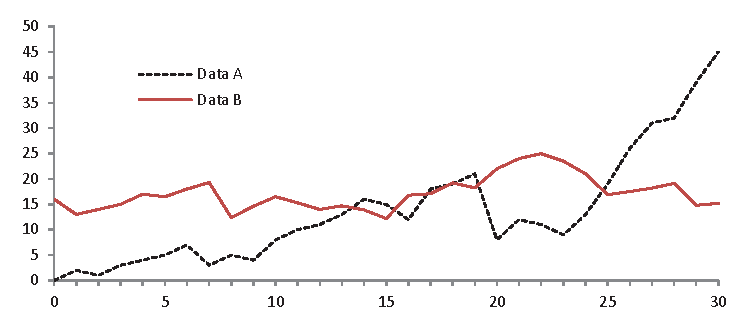
\includegraphics[width=\textwidth]{fig1.eps}
\caption{A figure caption is always placed below the illustration.
Please note that short captions are centered, while long ones are
justified by the macro package automatically.} \label{fig1}
\end{figure}

\begin{theorem}
This is a sample theorem. The run-in heading is set in bold, while
the following text appears in italics. Definitions, lemmas,
propositions, and corollaries are styled the same way.
\end{theorem}
%
% the environments 'definition', 'lemma', 'proposition', 'corollary',
% 'remark', and 'example' are defined in the LLNCS documentclass as well.
%
\begin{proof}
Proofs, examples, and remarks have the initial word in italics,
while the following text appears in normal font.
\end{proof}
For citations of references, we prefer the use of square brackets
and consecutive numbers. Citations using labels or the author/year
convention are also acceptable. The following bibliography provides
a sample reference list with entries for journal
articles~\cite{ref_article1}, an LNCS chapter~\cite{ref_lncs1}, a
book~\cite{ref_book1}, proceedings without editors~\cite{ref_proc1},
and a homepage~\cite{ref_url1}. Multiple citations are grouped
\cite{ref_article1,ref_lncs1,ref_book1},
\cite{ref_article1,ref_book1,ref_proc1,ref_url1}.
%
% ---- Bibliography ----
%
% BibTeX users should specify bibliography style 'splncs04'.
% References will then be sorted and formatted in the correct style.
%
% \bibliographystyle{splncs04}
% \bibliography{mybibliography}
%
\begin{thebibliography}{8}
\bibitem{1} Resnick P, Iacovou N, Suchak M, et al. GroupLens: an open architecture for collaborative filtering of netnews[C]// ACM Conference on Computer Supported Cooperative Work. ACM, 1994:175-186. (1994)

\bibitem{2} Sarwar B, Karypis G, Konstan J, et al. Item-based collaborative filtering recommendation algorithms[C]// International Conference on World Wide Web. ACM, 2001:285-295. (2001)

\bibitem{3} Chen YH, George EI. A Bayesian model for collaborative filtering. In: Proc. of the Int’l Workshop on Artificial Intelligence and Statistics. (1999)

\bibitem{4} Ungar LH, Foster DP. Clustering methods for collaborative filtering. In: Proc. of the AAAI Workshop on Recommendation
Systems. AAAI Press, 1998. 84−88 (1998)

\bibitem{5} Salakhutdinov R, Mnih A. Probabilistic matrix factorization[C]// International Conference on Machine Learning. 2008:880-887. (2008)

\bibitem{6} Balabanovi, Marko, Shoham Y. Fab: content-based, collaborative recommendation[J]. Communications of the Acm, 1997, 40(3):66-72. (1997)

\bibitem{7} Burke R. Hybrid Recommender Systems: Survey and Experiments[J]. User Modeling and User-Adapted Interaction, 2002, 12(4):331-370. (2002)

\bibitem{8} Dieleman S, Schrauwen B. Deep content-based music recommendation[C]// International Conference on Neural Information Processing Systems. Curran Associates Inc. 2013:2643-2651.(2013)

\bibitem{9} Okura S, Tagami Y, Ono S, et al. Embedding-based News Recommendation for Millions of Users[C]//Proceedings of the 23rd ACM SIGKDD International Conference on Knowledge Discovery and Data Mining. ACM, 2017: 1933-1942. (2017)

\bibitem{10} Covington P, Adams J, Sargin E. Deep Neural Networks for YouTube Recommendations[C]// ACM Conference on Recommender Systems. ACM, 2016:191-198. (2016)

\bibitem{11} Hidasi, Balázs, et al. "Session-based recommendations with recurrent neural networks." arXiv preprint arXiv:1511.06939 (2015)

\bibitem{12} Adomavicius G, Tuzhilin A. Toward the next generation of recommender systems: A survey of the state-of-the-art and possible extensions[J]. IEEE transactions on knowledge and data engineering, 2005, 17(6): 734-749. (2005)

\bibitem{13} Lai, Siwei, et al. "Recurrent Convolutional Neural Networks for Text Classification." AAAI. Vol. 333. 2015. (2015)

\bibitem{14} Sak H, Senior A, Beaufays F. Long short-term memory recurrent neural network architectures for large scale acoustic modeling[J]. Computer Science, 2014:338-342. (2014)

\bibitem{15} Wan S, Lan Y, Wang P, et al. Next Basket Recommendation with Neural Networks[C]//RecSys Posters. 2015. (2015)

\bibitem{16} Devooght R, Bersini H. Collaborative filtering with recurrent neural networks[J]. arXiv preprint arXiv:1608.07400, 2016. (2016)

\bibitem{17} Yu F, Liu Q, Wu S, et al. A dynamic recurrent model for next basket recommendation[C]//Proceedings of the 39th International ACM SIGIR conference on Research and Development in Information Retrieval. ACM, 2016: 729-732. (2016)

\bibitem{18} Ko Y J, Maystre L, Grossglauser M. Collaborative recurrent neural networks for dynamic recommender systems[C]//Asian Conference on Machine Learning. 2016: 366-381. (2016)

\bibitem{19} Jannach D, Ludewig M. When recurrent neural networks meet the neighborhood for session-based recommendation[C]//Proceedings of the Eleventh ACM Conference on Recommender Systems. ACM, 2017: 306-310. (2017)

\bibitem{20} Zhang S, Yao L, Sun A. Deep Learning based Recommender System: A Survey and New Perspectives[J]. arXiv preprint arXiv:1707.07435, 2017. (2017)

\bibitem{21} Bengio Y, Ducharme R, Vincent P, et al. A neural probabilistic language model[J]. Journal of machine learning research, 2003, 3(Feb): 1137-1155. (2003)
\bibitem{22} Ian Goodfellow, Yoshua Bengio, and Aaron Courville. 2016. Deep Learning. MIT Press. htp://www.deeplearningbook.org.
\end{thebibliography}
\end{document}
